\documentclass[12pt]{article}

\usepackage{tikz} % картинки в tikz
\usepackage{microtype} % свешивание пунктуации

\usepackage{array} % для столбцов фиксированной ширины

\usepackage{indentfirst} % отступ в первом параграфе

\usepackage{sectsty} % для центрирования названий частей
\allsectionsfont{\centering}

\usepackage{url}

\usepackage{amsmath, amssymb} % куча стандартных математических плюшек

\usepackage[top=2cm, left=1.5cm, right=1.5cm, bottom=2cm]{geometry} % размер текста на странице

\usepackage{lastpage} % чтобы узнать номер последней страницы

\usepackage{enumitem} % дополнительные плюшки для списков
%  например \begin{enumerate}[resume] позволяет продолжить нумерацию в новом списке
\usepackage{caption}


\usepackage{fancyhdr} % весёлые колонтитулы
\pagestyle{fancy}
\lhead{Теория вероятностей}
\chead{}
\rhead{2016-12-09, контрольная 2 :)}
\lfoot{}
\cfoot{}
\rfoot{\thepage/\pageref{LastPage}}
\renewcommand{\headrulewidth}{0.4pt}
\renewcommand{\footrulewidth}{0.4pt}



\usepackage{todonotes} % для вставки в документ заметок о том, что осталось сделать
% \todo{Здесь надо коэффициенты исправить}
% \missingfigure{Здесь будет Последний день Помпеи}
% \listoftodos — печатает все поставленные \todo'шки


% более красивые таблицы
\usepackage{booktabs}
% заповеди из докупентации:
% 1. Не используйте вертикальные линни
% 2. Не используйте двойные линии
% 3. Единицы измерения - в шапку таблицы
% 4. Не сокращайте .1 вместо 0.1
% 5. Повторяющееся значение повторяйте, а не говорите "то же"



\usepackage{fontspec}
\usepackage{polyglossia}

\setmainlanguage{russian}
\setotherlanguages{english}

% download "Linux Libertine" fonts:
% http://www.linuxlibertine.org/index.php?id=91&L=1
\setmainfont{Linux Libertine O} % or Helvetica, Arial, Cambria
% why do we need \newfontfamily:
% http://tex.stackexchange.com/questions/91507/
\newfontfamily{\cyrillicfonttt}{Linux Libertine O}



\AddEnumerateCounter{\asbuk}{\russian@alph}{щ} % для списков с русскими буквами
\setlist[enumerate, 2]{label=\asbuk*),ref=\asbuk*}


%% эконометрические сокращения
\renewcommand{\P}{\mathbb{P}}
\DeclareMathOperator{\Cov}{Cov}
\DeclareMathOperator{\Corr}{Corr}
\DeclareMathOperator{\Var}{Var}
\DeclareMathOperator{\E}{E}
\def \hb{\hat{\beta}}
\def \hs{\hat{\sigma}}
\def \htheta{\hat{\theta}}
\def \s{\sigma}
\def \hy{\hat{y}}
\def \hY{\hat{Y}}
\def \v1{\vec{1}}
\def \e{\varepsilon}
\def \he{\hat{\e}}
\def \z{z}
\def \hVar{\widehat{\Var}}
\def \hCorr{\widehat{\Corr}}
\def \hCov{\widehat{\Cov}}
\def \cN{\mathcal{N}}


\begin{document}


\textbf{Группа}\dotfill

\bigskip

\textbf{Ф.\,И.\,О.}\dotfill

\bigskip


\textbf{Неравенства Берри–Эссеена:} Для любых $n \in \mathbb{N}$ и всех $x \in \mathbb{R}$ имеет место оценка:
\[
    \bigl|F_{S_n^{*}}(x) - \Phi(x)\bigr| \leq 0.48 \cdot \frac{\E(|\xi_i - \E\xi_i|^3)}{\Var^{3/2}(\xi_i)\cdot\sqrt{n}} \text{,}
\]
где $\Phi(x) = \int_{-\infty}^{x}\frac{1}{\sqrt{2\pi}}e^{-\frac{t^2}{2}}\,dt$, \; $S_n^* = \frac{S_n - \E(S_n)}{\sqrt{\Var(S_n)}}$, \; $S_n = \xi_1 + \ldots + \xi_n$

\textbf{Распределение Пуассона:} Случайная величина $\xi$ имеет распределение Пуассона с параметром $\lambda > 0$,  если она принимает целые неотрицательные значения с вероятностями $\P(\{\xi = k\}) = \frac{\lambda^k}{k!}e^{-\lambda}$. Приличным студентам должно быть известно, что в этом случае $\E(\xi) = \Var(\xi) = \lambda$.

\begin{enumerate}
\item Пусть $\E(\xi) = 1$, $\E(\eta) = -2$, $\Var(\xi) = 1$, $\E(\eta^2) = 8$, $\E(\xi \eta) = -1$. Найдите
\begin{enumerate}
  \item{} [8] $\E(2\xi-\eta+1)$, $\Cov(\xi, \,\eta)$, $\Corr(\xi, \,\eta)$,  $\Var(2\xi-\eta+1)$;
  \item{} [8] $\Cov(\xi+\eta, \,\xi+1)$, $\Corr(\xi+\eta, \,\xi+1)$, $\Corr(\xi+\eta-24, \,365 - \xi - \eta)$, $\Cov(2016\cdot\xi, \, 2017)$.
\end{enumerate}

\item
Совместное распределение доходностей акций двух компаний задано с помощью таблицы:

\begin{center}
\begin{tabular}{c|cc}
\toprule
         & $\eta=-1$ & $\eta=1$ \\
\midrule
$\xi=-1$  & $0.1$       & $0.2$   \\
$\xi=0$   & $0.2$       & $0.2$   \\
$\xi=2$   & $0.2$       & $0.1$   \\
\bottomrule
\end{tabular}
\end{center}

\begin{enumerate}
  \item{} [2] Найдите частные распределения случайных величин $\xi$ и $\eta$.
  \item{} [2] Найдите $\Cov(\xi,\,\eta)$.
  \item{} [2] Сформулируйте определение независимости дискретных случайных величин.
  \item{} [2] Являются ли случайные величины $\xi$ и $\eta$ независимыми?
  \item{} [2] Найдите условное распределение случайной величины $\xi$, если $\eta = 1$.
  \item{} [2] Найдите условное математическое ожидание случайной величины $\xi$, если $\eta = 1$.
  \item{} [2] Найдите математическое ожидание и дисперсию величины $\pi = 0.5\, \xi + 0.5\, \eta$.
  \item{} [2] Рассмотрим портфель, в котором $\alpha$ — доля акций с доходностью $\xi$ и $(1 - \alpha)$ — доля акций с доходностью $\eta$. Доходность этого портфеля есть случайная величина
  \[\pi(\alpha) = \alpha \xi + (1-\alpha)\eta.\]
  Найдите такую долю $\alpha \in [0;\,1]$, при которой доходность портфеля $\pi(\alpha)$ имеет наименьшую дисперсию.
\end{enumerate}

\newpage
\item Число посетителей сайта \url{pokrovka11.wordpress.com} за один день имеет распределение Пуассона с математическим ожиданием 250.
\begin{enumerate}
  \item{} [2] Сформулируйте неравенство Маркова. При помощи данного неравенства оцените вероятность того, что за один день сайт посетят более 500 человек.
  \item{} [3] Сформулируйте неравенство Чебышева. Используя данное неравенство, определите наименьшее число дней, при котором с вероятностью не менее 99\% среднее за день число посетителей будет отличаться от 250 не~более чем на 10.
  \item{} [3] Решите предыдущий пункт с помощью центральной предельной теоремы.
  \item{} [2] Сформулируйте закон больших чисел. Обозначим через $\xi_i$ число посетителей сайта за $i$-ый день. Найдите предел по вероятности последовательности $\frac{\xi_1^2 + \ldots + \xi_n^2}{n}$ при $n \rightarrow \infty$.
\end{enumerate}

\item Отведав медовухи, Винни–Пух совершает случайное блуждание на прямой. Он стартует из начала координат и в каждую следующую минуту равновероятно совершает шаг единичной длины налево или направо. Передвижения Винни-Пуха схематично изображены на следующем рисунке.
\begin{figure}[h]
    \noindent\centering{
    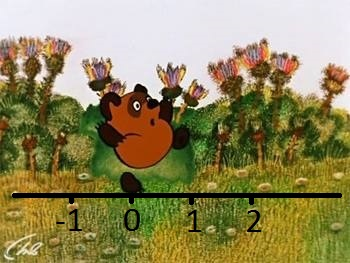
\includegraphics[width=80mm]{Winnie_the_Pooh_and_Medovuh.jpg}
    }
    \caption{Случайные бродилки.}
    \label{wun762hkej}
\end{figure}
\begin{enumerate}
  \item{} [1] Сформулируйте центральную предельную теорему.
  \item{} [6] При помощи центральной предельной теоремы оцените вероятность того, что ровно через час блужданий Винни-Пух окажется в области $(-\infty; \, -5]$.
  \item{} [3] Используя неравенство Берри–Эссеена оцените погрешность вычислений предыдущего пункта.
\end{enumerate}


\newpage
\item
Cлучайные величины $\xi$ и $\eta$ означают время безотказной работы рулевого управления и двигателя автомобиля соответственно. Время измеряется в годах. Совместная плотность имеет вид:
\[
f_{\xi, \,\eta}(x,\,y) =
\begin{cases}
0.005\,e^{-0.05\,x-0.1\,y} & \text{ при } x > 0, y > 0, \\
0                    & \text{ иначе.}
\end{cases}
\]

\begin{enumerate}
  \item{} [2] Найдите частные плотности распределения случайных величин $\xi$ и $\eta$.
  \item{} [1] Являются ли случайные величины $\xi$ и $\eta$ независимыми?
  \item{} [2] Найдите вероятность того, что двигатель прослужит без сбоев более пяти лет.
  \item{} [1] Найдите вероятность того, что двигатель прослужит без сбоев более восьми лет, если он уже проработал без сбоев три года.
  \item{} [2] Найдите условное математическое ожидание безотказной работы рулевого управления, если двигатель проработал без сбоев пять лет,  $\E(\xi | \eta = 5)$.
  \item{} [5] Найдите вероятность того, что рулевое управление проработает без сбоев на два года больше двигателя,  $\P(\{\xi - \eta > 2\})$.
\end{enumerate}

\item Бонусная задача

Случайная величина $\xi$ имеет плотность распределения
\[
    f_{\xi}(x) = \frac{1}{2} \cdot \frac{1}{\sqrt{2\pi}}e^{-\frac{(x-1)^2}{2}} + \frac{1}{2} \cdot \frac{1}{\sqrt{2\pi}}e^{-\frac{(x+1)^2}{2}} \text{.}
\]

\begin{enumerate}
\item{} [7] Найдите $\E(\xi)$, $\E(\xi^2)$, $\Var(\xi)$.
\item{} [3] Покажите, что функция $f_{\xi}(x)$, действительно, является плотностью распределения.
\end{enumerate}


\end{enumerate}


\begin{figure}[h]
    \noindent\centering{
    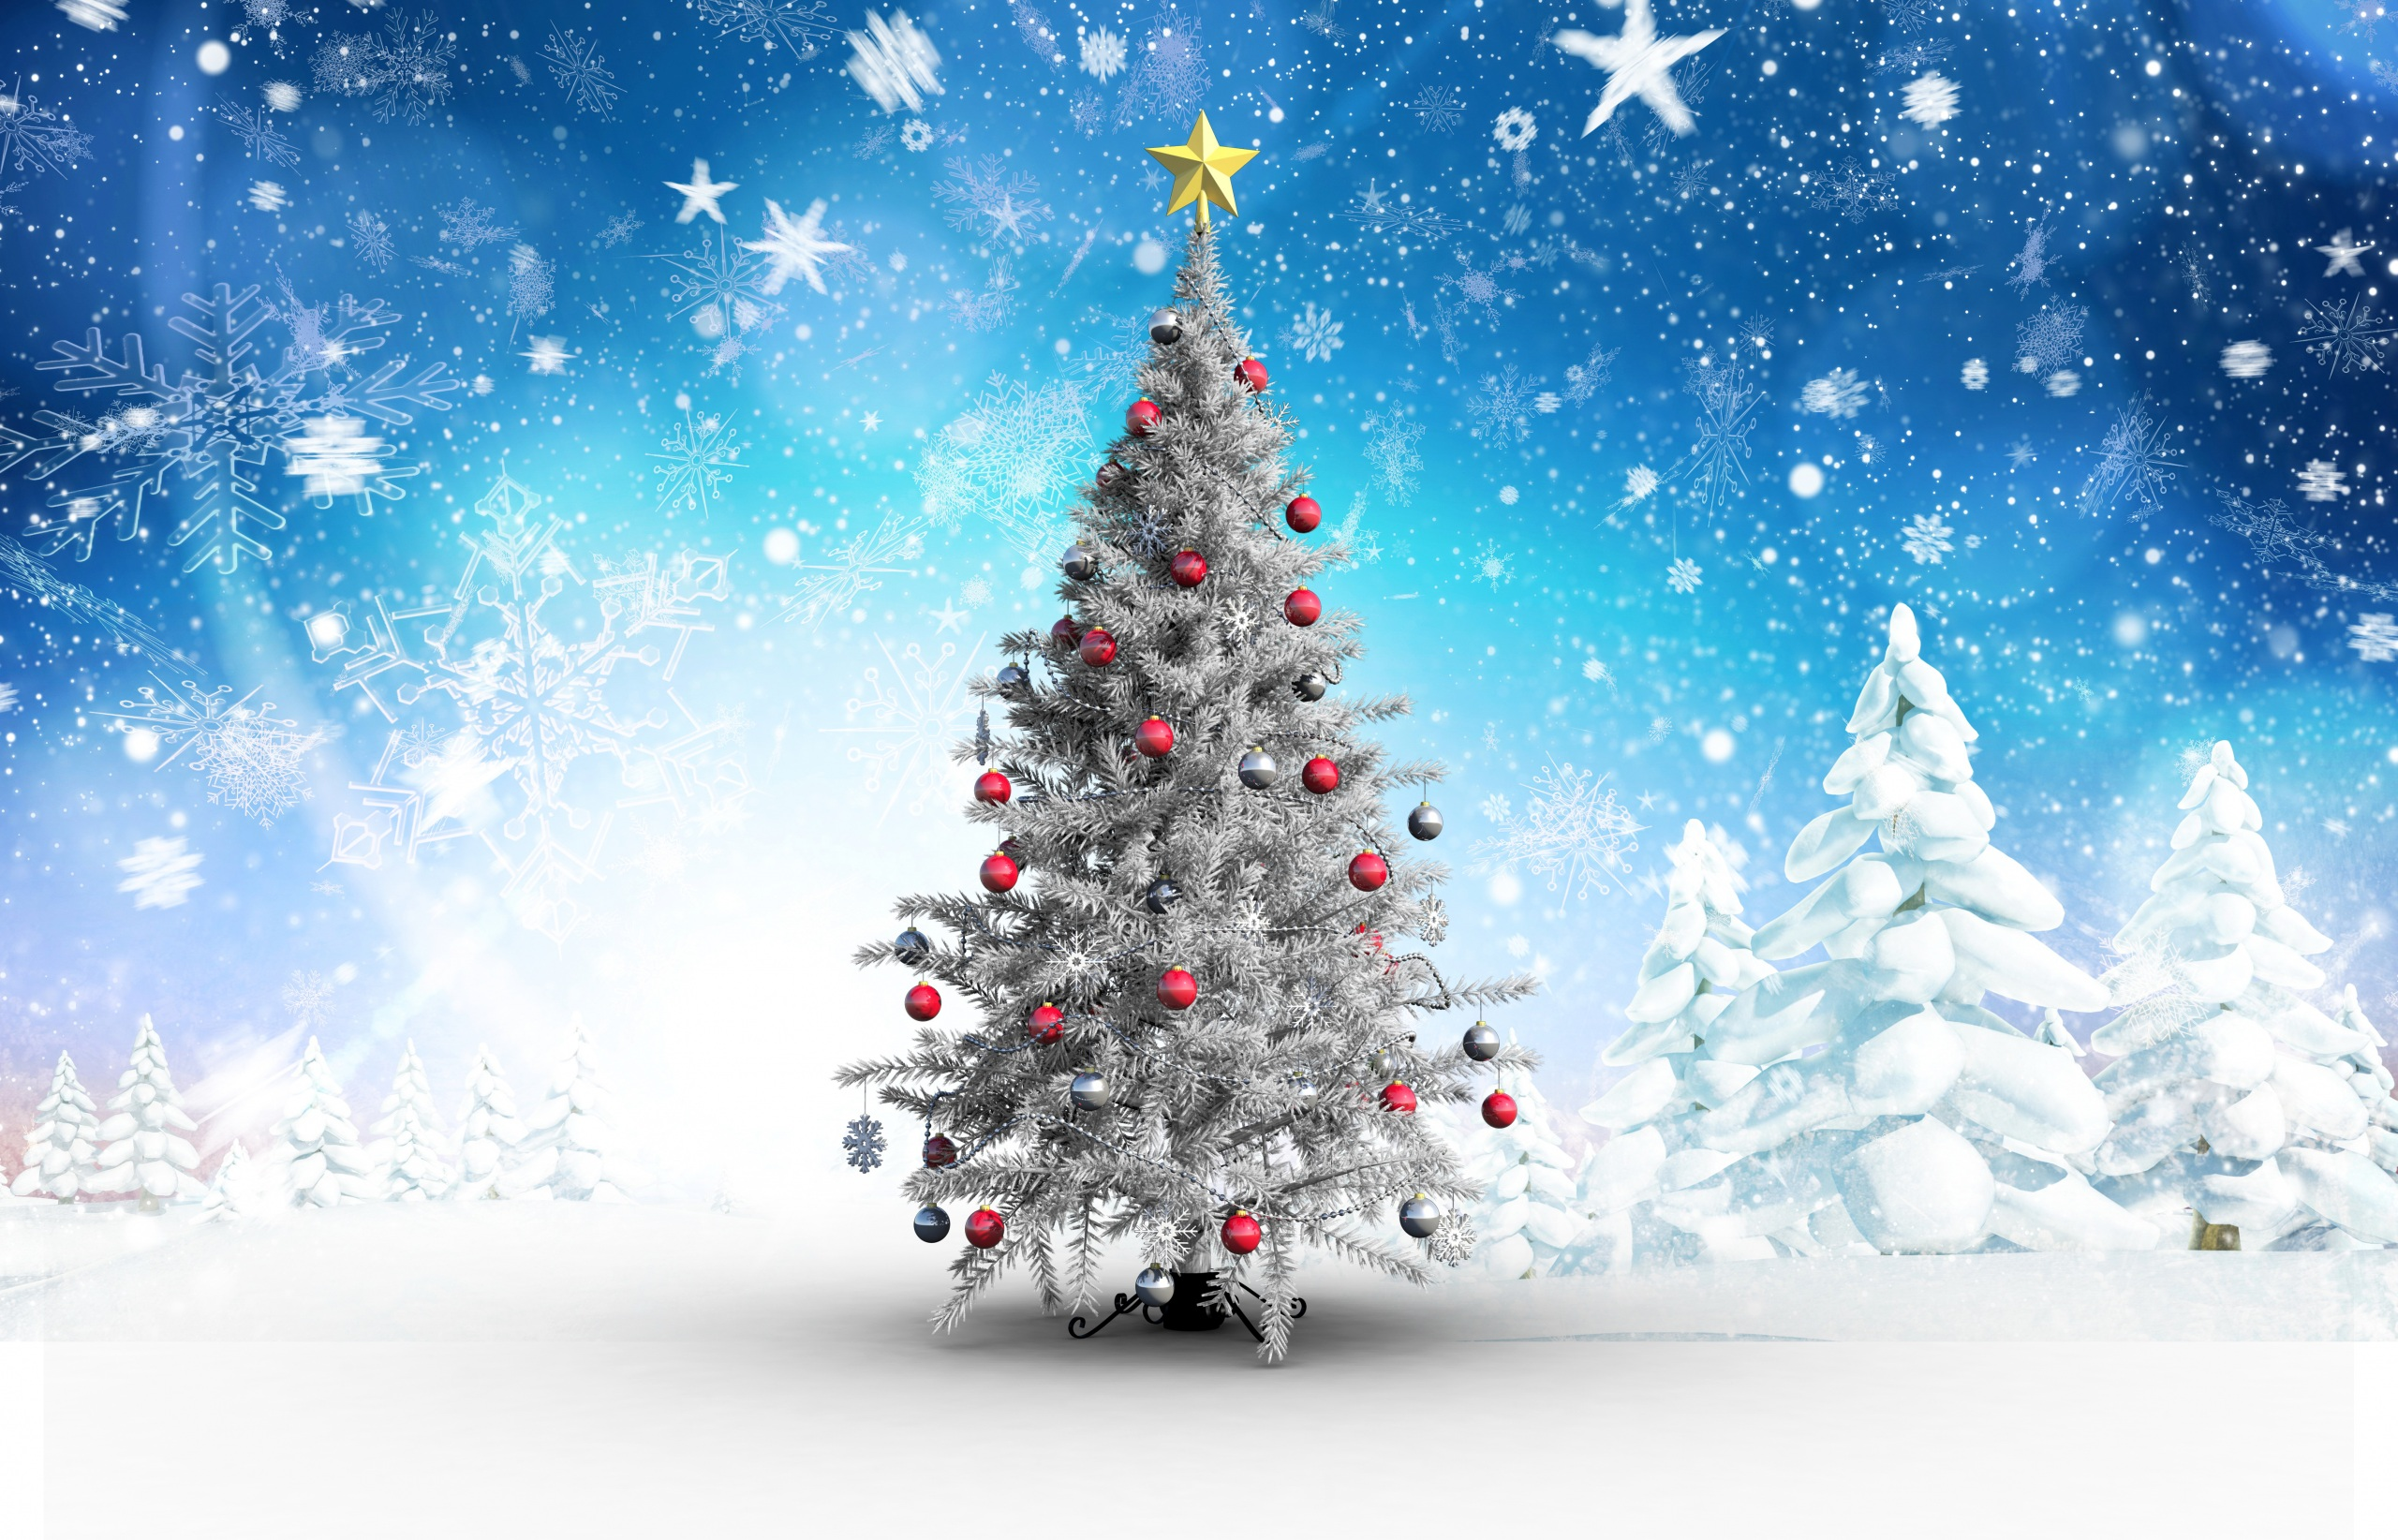
\includegraphics[width=80mm]{Holidays_Christmas_2016_2017.jpg}
    }
    \caption{Скоро Новый Год!!!}
    \label{sal8732h}
\end{figure}

\end{document}
